\documentclass{standalone}
\usepackage{tikz}
\usepackage{pgfplots}

\begin{document}


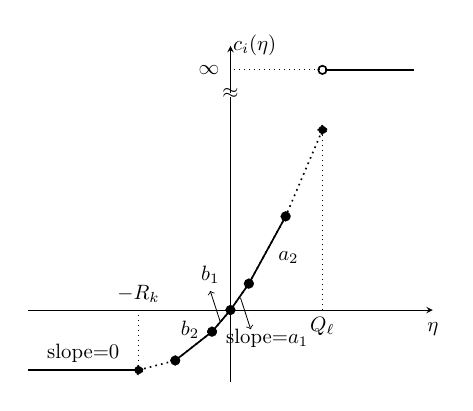
\begin{tikzpicture}[scale=.75]


\begin{axis}[axis lines=middle,
	xmin=-11,xmax=11,
         ytick=\empty,xtick=\empty,
         ymin=-3,ymax=11,  
         x label style={at={(axis description cs:1,.2)},anchor=north},
  	 y label style={at={(axis description cs:.56,.95)},anchor=south},
	 ylabel=$c_i(\eta)$,xlabel=$\eta$]
\addplot[samples at={-5,-3,-1,0,1,3,5},thick,dotted,mark=*] {.1*(x+5)^2-2.5};
\addplot[samples at={-3,-1,0,1,3},mark=*,thick] {.1*(x+5)^2-2.5};
\addplot[samples at={5},mark=o,thick] {10};
\addplot[samples at={5.15,10},mark=none,thick] {10};
\addplot[samples at={-5,-11},mark=none,thick] {-2.5};
\addplot[samples at={4.85,0},mark=none,dotted]{10};


\node at (axis cs:-.2,10) [left] {$\infty$};


\node at (axis cs:2,-.5) [below]{slope=$a_1$};
\draw[->] (axis cs:.55,.5) -- (axis cs:1.1,-.8);


\node at (axis cs:2.2,2.2) [right]{$a_2$};


\node at (axis cs:-1.1,.8) [above]{$b_1$};
\draw[->] (axis cs:-.55,-.5) -- (axis cs:-1.1,.8);


\node at (axis cs:-2.2,-1.5) [above]{$b_2$};


\node at (axis cs:-8,-2.5) [above]{slope=0};


\node at (axis cs:5,0) [below]{$Q_{\ell}$};
\draw[dotted] (axis cs:5,0) -- (axis cs:5,7.5);


\node at (axis cs:-5,0) [above]{$-R_{k}$};
\draw[dotted] (axis cs:-5,0) -- (axis cs:-5,-2.5);


\filldraw [color=white] (axis cs:-.2,8.9) rectangle (axis cs:.2,9);
\node at (axis cs:0,8.5) [above]{$\approx$};


\end{axis}


\end{tikzpicture}
\end{document}